\documentclass[tikz,border={0 3}]{standalone}

\usetikzlibrary{patterns,decorations.markings}

\def\lrad{1}
\def\mrad{0.175*\lrad}
\def\srad{0.15*\lrad}

\begin{document}
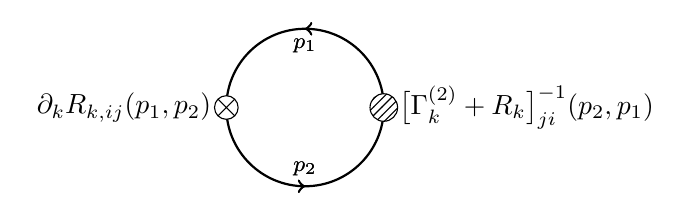
\begin{tikzpicture}[
    pin edge={shorten <=5*\lrad},
    cross/.style={fill=white,path picture={\draw[black] (path picture bounding box.south east) -- (path picture bounding box.north west) (path picture bounding box.south west) -- (path picture bounding box.north east);}},
    dressed/.style={fill=white,postaction={pattern=north east lines}},
    momentum/.style 2 args={->,semithick,yshift=5pt,shorten >=5pt,shorten <=5pt},
    loop/.style 2 args={thick,decoration={markings,mark=at position {#1} with {\arrow{>},\node[anchor=\pgfdecoratedangle-90,font=\footnotesize,] {$p_{#2}$};}},postaction={decorate}}
  ]

  \draw[loop/.list={{0.25}{1},{0.75}{2}}] (0,0) circle (\lrad);
  \draw[cross] (-\lrad,0) circle (\srad) node[left=2pt] {$\partial_k R_{k,ij}(p_1,p_2)$};
  \draw[dressed] (\lrad,0) circle (\mrad) node[right=2pt] {$\bigl[\Gamma_k^{(2)} + R_k\bigr]_{ji}^{-1}(p_2,p_1)$};

\end{tikzpicture}
\end{document}
